\chapter{Grundlagen und Stand der Technik}\label{ch:grundlagen}

Die moderne Robotik basiert auf einer Vielzahl von interagierenden Technologien der Signalverarbeitung, Objekterkennung und Modellgenerierung.

Die Basis dieses Technologiestapels bildet die Erfassung und Erkennung der Gegebenheiten der echten Welt und ihre Verarbeitung, Verteilung und Auswertung innerhalb eines informationstechnischen Frameworks.

Dabei kommen Technologien wie beispielsweise Laserscanner, Time-Of-Flight-Kamera, Musterprojektion, sowie Mono- und Stereokameras kombiniert mit Analyseverfahren zur Erkennung von einzelnen Objekten, beispielsweise Markern, Stühlen, Tischen, Tellern oder Tassen zum Einsatz.
Da sich diese Arbeit vorwiegend auf die letztgenannten Mono- und Stereokameras kombiniert mit Bilderkennungsverfahren stützt, werden im folgenden die damit verbundenen Verfahren und Technologien näher erläutert.
Anschließend folgt eine kurze Einführung in die verwendeten mathematischen Formalismen wie zum Beispiel Quaternionen und ihre Anwendung innerhalb des Systems.

Integriert werden alle Komponenten mit Hilfe der vom Robot Operating System(ROS) bereitgestellten Hilfsmittel.

\section{Robot Operating System(ROS)}

\begin{figure}
  \centering
  \includegraphics[width=0.4\textwidth]{bilder/pr2.jpg}
  \caption{PR2 von Willow Garage}
  \label{fig:pr2}
\end{figure}

Entwickelt von dem in den USA ansässigen privaten Forschungslabor "`Willow Garage"' stellt das Robot Operating System\betterfootcite{quigley2009ros} eine Abstraktions- und Vermittlungsschicht für unterschiedlichste Komponenten eines Robotersystems bereit.
Es fungiert dabei als eine Art Metabetriebssystem, welches lokale und entfernte Kommunikation harmonisiert, einfache Werkzeuge zur Verwaltung großer Softwareprojekte bereitstellt sowie essentielle Komponenten für alltägliche Robotikaufgaben, wie zum Beispiel Kamerasteuerung und Kalibrierung, mitliefert.
Das Aushängeschild von "`Willo Garage"', der Roboter "`PR2"' in Abbildung \vref{fig:pr2} wird beispielsweise mit dem Robot Operating System betrieben.

\subsection{Struktur}
Die Grundkomponenten des Robot Operating Systems bestehen aus dem ROS-Master und einem oder mehreren ROS-Knoten.
Der ROS Master ist die zentrale Koordinationsinstanz des Systems und vermittelt zwischen den einzelnen Knoten.
Jeder Knoten im ROS ist ein separater Prozess des Hostbetriebssystems, welcher über die bereitgestellte ROS-Programmbibliothek mit dem Master und den anderen Knotens kommuniziert.
Der Master fungiert dabei ausschließlich als Vermittler und als zentrale Anlaufstelle für Metadaten des Gesamtsystems.
Dabei können innerhalb des Gesamtsystems einzelne Knoten in Namensräume der Form "`/recognizer/shape\_based\_recognizer"' verteilt werden um eine einfache namentliche Adressierung der Knotens zu ermöglichen.

\subsection{Netzwerkvermittlung}

Eine der Kernkomponenten von ROS ist die Nachrichtenvermittlung zwischen verschiedenen Knoten.
Diese läuft primär über zwei verschiedene Modi ab, kommuniziert aber in jedem Fall mittels vorher definierter Nachrichtentypen.
Diese Nachrichtentypen müssen schon zur Kompilierungszeit allen Komponten bekannt sein und erlauben einen Datenaustausch über System und Programmiersprachengrenzen hinweg.

\subsubsection{Publisher/Subscriber-Kommunikation}

Das verbreitetste Kommunikationsverfahren basiert auf dem Publisher/Subscriber-Muster, welches in Abbildung \vref{fig:pubsub} illustriert ist.

Dabei informiert ein Knoten, hier genannt Publisher, den Master, dass er Nachrichten eines bestimmten Typs an ein sogenanntes "`Topic"' verbreitet.
Dieses Topic ist identifiziert mit einem String, welcher optional relativ zur Position des veröffentlichenden Knotens im ROS-Namensraum aufgefasst werden kann.
Wenn nun ein zweiter Knoten die Nachrichten eines Topics abonnieren will, benachrichtigt er den Master.
Dieser teilt dem zuständigen Publisher die Identität des Abonnenten mit, wodurch der Publisher in der Lage ist alle Nachrichten direkt an den Empfänger zu versenden.
Dieser Mechanismus ermöglicht eine dezentrale Verteilung des Netzwerkverkehrs, was bei großen Übertragungsvolumina einen einzelnen Flaschenhals vermeidet.
Hierbei ist noch anzumerken dass diese Form der Kommunikation nicht auf eine 1-zu-1-Beziehung beschränkt ist.
Es können für das gleiche Topic sowohl mehrere Publisher als auch mehrere Subscriber vorhanden sein.
Das Verhalten ist jedoch in jedem Fall analog.

\begin{figure}
  \centering
  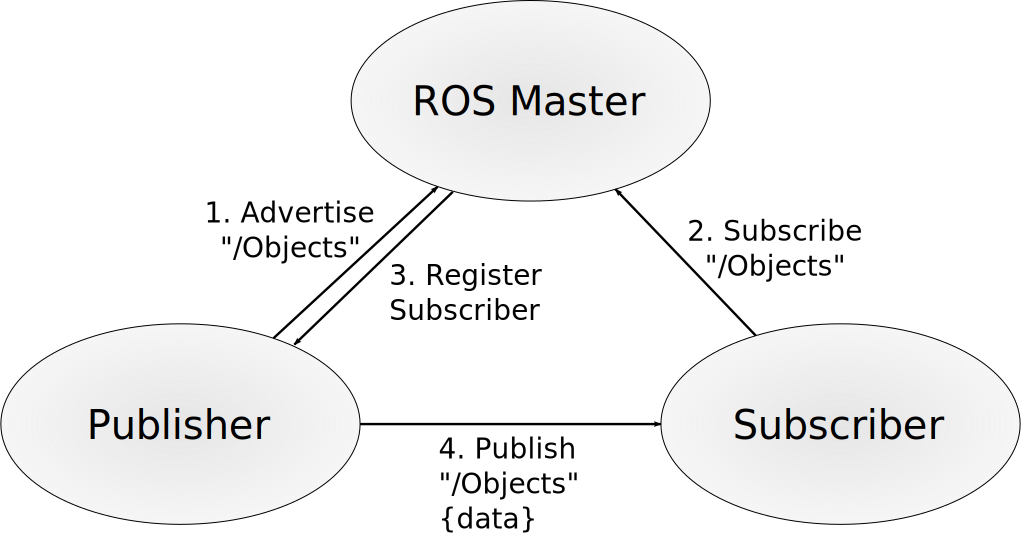
\includegraphics[width=0.7\textwidth]{bilder/pubsub.pdf}
  \caption{Publisher/Subscriber-Muster}
  \label{fig:pubsub}
\end{figure}

\subsubsection{Service-Kommunikation/Remote Procedure Calls}
Als Alternative zu der n-zu-m-Kommunikation des Publisher/Subscriber-Systems existiert ein Service-Modell, welches es ermöglicht direkte Anfragen an einzelne Knoten zu stellen.
Dieser Modus wird häufig benutzt um direkte Befehle zwischen speziellen Komponenten auszutauschen.
Ein Beispiel dafür wäre zum Beispiel die Ansteuerung bestimmter Motoren zur Fortbewegung des Roboters oder Änderung der Blickrichtung des Roboterkopfes.
Das Verfahren ist dem Ablauf der Publisher/Subscriber-Kommunikation sehr ähnlich. Der Serviceanbieter teilt dem Master-Knoten mit, welche Servicefunktionen er bereitstellt.
Diese können von Klienten abgefragt und direkt bei dem zuständigen Serviceknoten aufgerufen werden.
ROS abstrahiert die einzelnen Aufrufe auf eine Art und Weise, die an das Aufrufen nativer Funktionen des Klientencodes ähnelt um einfache Integration in das verteilte System zu ermöglichen.

\section{Objekterkennung}

Die Objekterkennung ist ein wertvolles Mittel bei der Szenenerkennung, da sie eine Basis für eine abstraktere Verarbeitung der wahrgenommenen Zusammenhänge bildet.
Sie ist besonders bei der Szenenerkennung in Innenräumen hilfreich, da die direkte Ausgabe von Koordinaten und Orientierungen erkannter Objekte die Weiterverarbeitung in einem geometrischen Kontext erleichtert.
Allgemein werden bei der Objekterkennung ausgehend von Sensordaten wie beispielsweise Punktwolken, Mono- oder Stereobildern mit Hilfe von Bildverarbeitungsverfahren abstrakte Merkmale extrahiert, diese werden anschließend in durch die eigentlichen Objekterkenner interpretiert, woraus dreidimensionale Informationen über gesehen Objekte erlangt werden, welche unabhängig von den Erkennungsmodalitäten weiterverarbeitet werden können.
Im Folgenden werden die in dieser Arbeit verwendeten Objekterkennungsverfahren näher erläutert.

\subsection{Markererkennung}

Die Markererkennung basiert auf der Erkennung quadratischer Marker fester Größe, welche mit vorher generierten Mustern versehen sind.
Aus Größe und Form des gesehen Markers in Kombination mit den passenden Kamerakoordinaten können die sechsdimensionalen Posen der Marker sehr zuverlässig erkannt werden.
Eine Illustration der Markererkennung ist in Abbildung \vref{fig:marker} ersichtlich.
Leider ist diese Form der Erkennung äußerst anfällig für Überdeckungen, weswegen sie für einen realistischen Einsatz mit anderen Erkennungssystemen kombiniert werden muss.
Das eingesetzte System basiert auf der Markererkennung des Karlsruhe Institut für Technologie-Spinoffs Keyetech.

\begin{figure}
  \centering
  \includegraphics[width=0.6\textwidth]{bilder/marker.jpg}
  \caption{Markererkennung: Zu sehen sind sowohl verdeckte als auch erkannte Marker.}
  \label{fig:marker}
\end{figure}

\subsection{Texturbasierte Erkennung}

Als zuverlässiges Erkennungsverfahren für flächige Objekte mit einer einzigartigen Textur, wie zum Beispiel Cornflakes-Packungen, wurde eine an der Universität Karlsruhe entwickelte Texturerkennung\betterfootcite{Azad:2009:CHI:1732643.1732747} verwendet.\\
Diese benutzt eine Kombination aus SIFT-Features\betterfootcite{lowe2004distinctive} und Harris Interest Points\betterfootcite{harris1988combined} um eine robuste, skalierungsinvariante Erkennung zu ermöglichen.

Dafür wird zunächst ein neuer Featuretyp auf Basis der SIFT-Features and Harris Interest Points definiert.
Die aus Vorlagen extrahierten Features werden bei der Erkennung zunächst in einen Hough-Voting-Verfahren aggregiert.
Der resultierende Hough-Raum wird mit Hilfe des RANSAC-Verfahrens\betterfootcite{Fischler:1981:RSC:358669.358692} von Ausreißern bereinigt.
Für die verbleibenden Features wird mittels der Methode der kleinsten Quadrate in einem iterativen Verfahren versucht eine affine Abbildung zu finden sodass die erkannten Features der Originalkonstellation entsprechen.
In diesem Verfahren werden abermals schrittweise Ausreißer entfernt.
Sollten am Ende noch genug valide Features verbleiben, so wird das entsprechende Objekt als erkannt markiert.
Da dem Erkennungsverfahren auch die Objektgeometrie vorliegt, ermöglicht die Erkennung einer texturierten Seite eines Objektes automatisch die Erkennung des gesamten Objektes inklusive der Position und Orientierung im Raum.

\subsection{Objektgeometriebasierte Erkennung}

Ebenfalls von der Universität Karlsruhe entwickelt, gewährleistet die Geometriebasierte Erkennung einfarbiger Objekte\betterfootcite{conf/iros/AzadAD09} eine robuste und genaue Erkennung\betterfootcite{azad20116}.
Sie basiert auf dem Segmentieren der einfarbigen Objekte in Stereo-Kamerabildern.
Auf das segmentierte Objekt wird dann ein Canny-Kantendetektor\betterfootcite{canny1986computational} angewandt um die Form des Objektes zu ermitteln.
Dann wird versucht ein Bild des Objektes auf Basis vorhandener 3D-Modelle aus einer ähnlichen Pose zu rendern.
Auf das resultierende gerenderte Bild wird der gleiche Kantendetektor angewandt.

Mit Hilfe eines sequentiellen Monte-Carlo-Verfahrens\betterfootcite{halton1967sequential}, wird anschließend versucht das gerenderte Bild mit dem Originalbild bezüglich der erkannten Kanten in Einklang zu bringen.
Als Maß für den Fehler zwischen dem Original Kantenbild $I_g$ und dem Kantenbild des gerenderten Bildes $I_{g,p}$ wird dabei folgende Formel verwendet:
\begin{equation}
 w_g(I_g, I_{g,p}) = 1 - \frac{\sum_{x,y} \left[ I_g(x,y) \text{ AND } I_{g,p}(x,y) \right]}{\sum_{x,y} I_{g,p}(x,y)}
\end{equation}

Wobei "`AND"' das binäre "`Und"' bezeichnet.

Wenn dies erfolgreich war, kann mit Hilfe der Render- und Kameraparameter die Ausrichtung und Entfernung des Objektes relativ zur Kamera bestimmt werden.
Eine Illustration des Ablaufes ist in Abbildung \vref{fig:shape-recognition} dargestellt.

\begin{figure}
  \begin{center}
    \begin{subfigure}[b]{.3\textwidth}
      \includegraphics[width=1\linewidth]{bilder/shape/-008.jpg}
    \end{subfigure}
    \begin{subfigure}[b]{.3\textwidth}
      \includegraphics[width=1\linewidth]{bilder/shape/-006.jpg}
    \end{subfigure}\\
    \begin{subfigure}[b]{.3\textwidth}
      \includegraphics[width=1\linewidth]{bilder/shape/-007.jpg}
    \end{subfigure}
    \begin{subfigure}[b]{.3\textwidth}
      \includegraphics[width=1\linewidth]{bilder/shape/-026.jpg}
    \end{subfigure}
  \end{center}
  \caption{Objektgeometriebasierte Erkennung. Bildquelle: \cite{azad20116}}\label{fig:shape-recognition}
\end{figure}

\section{Implicit Shape Models (ISMs)}

Implicit Shape Models bilden die Basis des entwickelten Systems.
Sie basieren auf der generalisierten Hough-Transformation\betterfootcite{ballard1981generalizing}.
Das Grundprinzip von Implicit Shape Models beruht auf dem Ansatz der Wiedererkennung eines größeren Zusammenhangs anhand seiner Teile.
Beispielsweise werden für die Erkennung eines Stuhls die einzelnen Stuhlteile, erkannt und aus den Lageinformationn diese Teile, wie zum Beispiel Stuhlbeine, Sitzfläche, Lehne etc., inferiert, ob es sich um einen Stuhl handelt, und wenn ja, wo er sich befindet.
Dabei ist diese Modellart keineswegs nur auf leblose Gegenstände begrenzt.
Implicit Shape Models werden beispielsweise auch für die Erkennung von Fußgängern (Abbildung \vref{fig:pedestrians}) in zweidimensionalen Aufnahmen benutzt, in denen sie auf der Erkennung einzelner Körperteile, wie zum Beispiel Füßen, Armen und Kopf beruhen.

\begin{figure}
  \begin{centering}
    \begin{subfigure}[b]{.3\textwidth}
      \includegraphics[width=1\linewidth]{bilder/pedestrian/pedest-000.jpg}
    \end{subfigure}
    \begin{subfigure}[b]{.3\textwidth}
      \includegraphics[width=1\linewidth]{bilder/pedestrian/pedest-001.jpg}
    \end{subfigure}
    \begin{subfigure}[b]{.3\textwidth}
      \includegraphics[width=1\linewidth]{bilder/pedestrian/walk-annotation.pdf}
    \end{subfigure}
  \end{centering}
  \caption{Fußgängererkennung mittels Implicit Shape Models. Bildquelle: \cite{pedestrian}}\label{fig:pedestrians}
\end{figure}


\subsection{Training}

Für das Training von Implicit Shape Models sind vorher annotierte Eingabedaten notwendig.
Diese umfassen die Position und Orientierung des zu erkennenden Objektes sowie die Positionen der einzelnen Objektteile.
Anhand der Eingabedaten wird im ersten Schritt ein Codebuch generiert, welches Informationen über die Position und Lage einzelner Teile eines zu erkennenden Objektes enthält.
Ein Beispiel eines Codebuches ist im zweiten Bild in Abbildung \vref{fig:pedestrians} zu erkennen.
Mittels dieses Codebuches werden die Lagen der einzelnen Teile eines Objektes relativ zu einem Referenzpunkt vermerkt.
Dieser Referenzpunkt ergibt sich im Allgemeinen aus dem Mittelpunkt aller Teile des zu erkennen Objektes, kann jedoch auch an die Position eines beliebigen Teils des Gesamtobjektes gesetzt werden.

Beispielhaft wird die Fahrzeugerkennung verwendet: \\
Die Eingabedaten bestehen aus einer Reihe von Fahrzeugbildern.
Jedes Bild ist annotiert mit dem Mittelpunkt des Fahrzeugs sowie, beispielsweise, mit den Positionen der Räder.
Aus all diesen Bildern wird nun ein Codebuch generiert.
Dafür betrachtet man jedes einzelne Teilobjekt in den Eingabedaten, wie etwa, alle Räder einer bestimmten Form in allen Bildern.
Für diese spezielle Form wird ein neuer Codebucheintrag angelegt.
Er enthält die Beschreibung der Form des Rades und eine Liste.
Die Einträge in dieser Liste sind für jedes Auftreten des Teils in einem Bild der Vektor, welcher von diesem Teil relativ zur Orientierung des Teils zum Referenzpunkt des Fahrzeugs zeigt.
Dieser repräsentiert die relative Lage des Fahrzeugteils zum Mittelpunkt des Fahrzeugs.
Danach enthält das Codebuch eine Sammlung von einzelnen zu erkennenden Fahrzeugteilen und jeweils eine Liste von relativen Vektoren zum Mittelpunkt des Fahrzeugs.

\subsection{Erkennung}

\begin{figure}
  \centering
  \includegraphics[width=1.0\textwidth]{bilder/ISM/leibe-car.jpg}
  \caption{Erkennung eines Fahrzeugs mit anschließender Segmentierung. Bildquelle:~\textcite{Leibe04combinedobject}.}
  \label{fig:leibe-car}
\end{figure}

Um nun ein Objekt mittels eines vorher angelegten Codebuches wiederzuerkennen sind folgende Schritte notwendig:

\begin{itemize}
\item Erkennen der einzelnen Teile des Objektes in den Eingabedaten mit Hilfe ihrer Beschreibungen aus dem Codebuch.
\item Anlegen aller relativen zu dem Objektteil gehörenden Vektoren aus dem Codebuch an die gefunden Teile.
\item Ermitteln eines lokalen Maximums eingehender Vektoren.
\end{itemize}

Dabei gibt es eine Vielzahl von Methoden um das lokale Maximum eingehender Vektoren zu bestimmen.
Das in dieser Arbeit verwendete Verfahren verwendet eine Diskretisierung des Raumes in Buckets, in welchen die Vektoren aggregiert werden.
Dies kann entweder durch eine naive Suche des größten Buckets geschehen, oder mit erweiterten Methoden wie des Best-Bin-First Algorithmus\betterfootcite{Beis97shapeindexing}\betterfootcite{lowe1999object}.
Es ist jedoch auch möglich eine Maximumssuche in einem kontinuierlichen Raum durchzuführen, beispielsweise mittels  k-means Clustering\betterfootcite{zbMATH03340881} oder Mean-Shift-Mode Estimation\betterfootcite{cheng1995mean}.
Nachdem eine lokales Maximum gefunden wurde, kann daraus geschlossen werden, dass sich an dieser Position das gewünschte Objekt befindet.

Dies soll nun nochmals am Beispiel einer Fahrzeugerkennung erläutern werden:

Als Eingabe wird ein unbekanntes Bild eines Fahrzeugs gegeben.
Es wird nun versucht anhand des Codebuches die einzelnen Teile des Fahrzeugs wiederzuerkennen.
Wenn beispielsweise ein Rad erkannt wird, werden an dessen Position alle vorher gefundenen Vektoren zu möglichen Referenzpunkten angelegt.
Daraus ergibt sich eine Häufung eingehender Vektoren im Zentrum des abgebildeten Fahrzeugs und es kann daraus geschlussfolgert werden, dass sich an dieser Stelle eine Fahrzeug befindet.
Dies ist in Abbildung \vref{fig:leibe-car} beispielhaft zu erkennen.

\subsection{Probleme}\label{ch:ISM-Probleme}

Der naive Implicit Shape Model Ansatz versagt leider in einigen wichtigen Szenarien.
Eines dieser Probleme, "`Vertauschungsproblem"' genannt, soll hier kurz erläutert werden.
Das Vertauschungsproblem tritt in folgender Situation auf:

Angenommen es werden drei Objekte betrachtet.
Eines von ihnen, Objekt A, liegt zentral, ist statisch und wird als Referenzpunkt angenommen.
Die anderen Objekte, B1 und B2, sind jeweils Objekte das gleichen Typs und bewegen sich in konstantem Abstand zueinander an Objekt A vorbei.
Diese Situation ist in Abbildung \vref{fig:vertauschung} dargestellt.
Wie deutlich wird, führt die Erkennung der zweiten Trainingssituation zu einer Doppeldeutigkeit, da sowohl B1 als auch B2 in beiden B-Positionen gesehen wurden.
Im Zuge dieser Arbeit ist eine Strategie erarbeitet worden, um diese Probleme des Implicit Shape Models zu erkennen und zu lösen.

\begin{figure}
  \centering
  \includegraphics[width=1\textwidth]{bilder/vertauschungsproblem.pdf}
  \caption{Illustration des Vertauschungsproblems}
  \label{fig:vertauschung}
\end{figure}

\section{Stand der Technik}

Bisherige Verfahren verwenden Implicit Shape Models unter anderem zur Erkennung von Objekten wie Fahrzeugs oder Fußgängern in zweidimensionalen Bildern\betterfootcite{Leibe04combinedobject}.
Es existieren auch bereits Ansätze für eine Erkennung von Dreidimensionalen Objekten innerhalb von Punktwolken\betterfootcite{implicitShape3dPointClouds}.
\citeauthor{wittrowski20133d}\betterfootcite{wittrowski20133d} beschreiben ein System zur Erkennung von Möbelstücken wie beispielsweise Stühlen in Punktwolken anhand von ISMs.
Jedoch ist dem Autor momentan kein System bekannt, welches versucht dynamische Szenen mit Hilfe von Implicit Shape Models zu erkennen.

Zur Szenenerkennung gibt es weitere nicht auf Implicit Shape Models basierende Verfahren.
Pyramid Matching Kernel\betterfootcite{grauman2005pyramid} und darauf aufbauende Spatial Pyramid Mathing Kernel \betterfootcite{lazebnik2006beyond} extrahieren lokale Features aus 2D Bildern und benutzen bereits ihre relativen Positionen zueinander zum bestimmen der Szenentypen.
\citeauthor{5509682}\betterfootcite{5509682} verwenden ein Sliding-Window verfahren zur direkten Erkennung von Objekten wie beispielsweise Computermonitoren in zweidimensionalen Bilddaten zur Klassifikation der Szene anhand vorhandener Objekte.
\citeauthor{cakir2011nearest}\betterfootcite{cakir2011nearest} schlagen einen ähnlichen Ansatz vor, welcher Nachbarschaftsbeziehungen zwischen signifikanten Bildausschnitten welche durch SIFT-Features gewählt werden.